%%==================================================
%% chapter03.tex for SJTU Master Thesis
%% Encoding: UTF-8
%%==================================================

\chapter{实验与结果分析}
\label{chap:experiment}

在这一章节中,我们将会给出应用本文提出的流体动画重构上采样框架的流体动画模拟效果图。为了探讨本文的流体动画重构上采样方法在流体动画领域的适用性与可行性,本文将会展示使用Yang的重构上采样算法与本文给出的重构上采样方法的对比实验。另外,为了说明本文重构上采样方法的重构结果的准确性,我们也会给出该重构上采样方法在图像超分辨领域的实验。

\section{L1SR和scSR重构上采样方法与框架}

\subsection{实验目的与环境}

该部分实验的目的是观察并验证本文提出的基于过完备稀疏训练字典方法的流体动画计算框架的可行性,并探索可能存在的问题,为后续的研究工作做好调研工作。

该部分的实验在Matlab环境下开发,实验用的机器的内核是Intel Core i7 3.40G,内存为16G。实现Bridson~\cite{bridson2007fluid}的流体模拟器作为本文流体模拟的基本框架,对流部分采用经典的半拉格朗日方法,投影步骤求解压强场的矩阵线性方程使用的的雅可比迭代器求解。使用L1SR方法重构上采样流体的局部细微结构时,代表流体局部细微结构的patch的大小设置为$3\times3$;在应用scSR重构上采样流体局部细微结构时,则使用patch的大小为$5\times5$。在用L1SR或scSR方法重构上采样流体低精度速度场数据时,考虑到稀疏表示的训练字典最优空间与重构最优空间不一致,故在训练字典的过程中,设置拉格朗日算子$\lambda$的值为0.15,而在重构时去对应的拉格朗日算子$\lambda$的值为0.2。另外,在实验中,我们设置流体速度场的放大因子为2,训练字典的大小为512(即每一个字典有512个原子项),高精度的流体场的网格精度为$512\times512$。

\subsection{实验结果与分析}

\begin{figure}[!ht]
  \centering
  
\includegraphics[width=0.23\textwidth]{chap5/L1SR/high_res256d40}
  \hspace{0.1cm}
  
\includegraphics[width=0.23\textwidth]{chap5/L1SR/bic_res256d40}
   \hspace{0.1cm}
  
\includegraphics[width=0.23\textwidth]{chap5/L1SR/L1SR_05_res256d40}
   \hspace{0.1cm}
  
\includegraphics[width=0.23\textwidth]{chap5/L1SR/L1SR_07_res256d40}
  
  \vspace{0.1cm}  
   
\includegraphics[width=0.23\textwidth]{chap5/L1SR/high_res256d55}
  \hspace{0.1cm}
  
\includegraphics[width=0.23\textwidth]{chap5/L1SR/bic_res256d55}
   \hspace{0.1cm}
  
\includegraphics[width=0.23\textwidth]{chap5/L1SR/L1SR_05_res256d55}
   \hspace{0.1cm}
  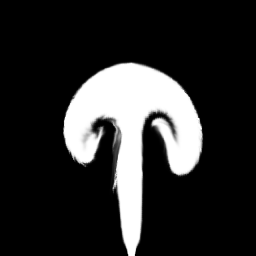
\includegraphics[width=0.23\textwidth]{chap5/L1SR/L1SR_07_res256d55}
  
    \vspace{0.1cm}  
   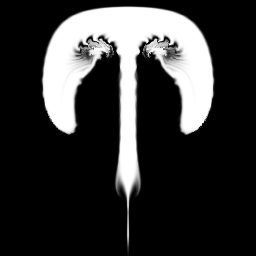
\includegraphics[width=0.23\textwidth]{chap5/L1SR/high_res256d62}
  \hspace{0.1cm}
  
\includegraphics[width=0.23\textwidth]{chap5/L1SR/bic_res256d62}
   \hspace{0.1cm}
  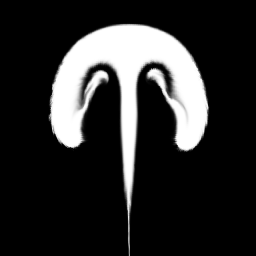
\includegraphics[width=0.23\textwidth]{chap5/L1SR/L1SR_05_res256d62}
   \hspace{0.1cm}
  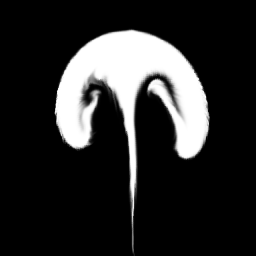
\includegraphics[width=0.23\textwidth]{chap5/L1SR/L1SR_07_res256d62}
  
    \vspace{0.1cm}  
   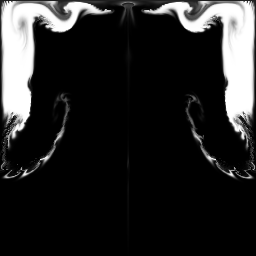
\includegraphics[width=0.23\textwidth]{chap5/L1SR/high_res256d88}
  \hspace{0.1cm}
  
\includegraphics[width=0.23\textwidth]{chap5/L1SR/bic_res256d88}
   \hspace{0.1cm}
  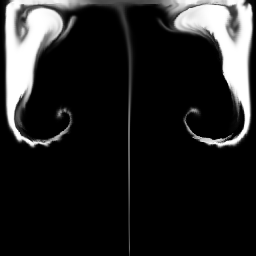
\includegraphics[width=0.23\textwidth]{chap5/L1SR/L1SR_05_res256d88}
   \hspace{0.1cm}
  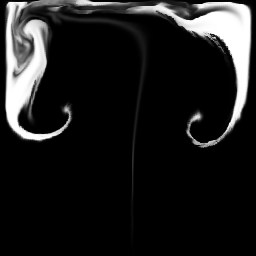
\includegraphics[width=0.23\textwidth]{chap5/L1SR/L1SR_07_res256d88}
   \newline  (a) \ \ \ \ \ \ \ \ \ \ \ \ \ \ \ \ \ \ \ \ \ \ \ \ \ \ \ \ \ \ (b) \ \ \ \ \ \ \ \ \ \ \ \ \ \ \ \ \ \ \ \ \ \ \ \ \ \ \ (c) \ \ \ \ \ \ \ \ \ \ \ \ \ \ \ \ \ \ \ \ \ \ \ \ \ \ \ \ \ \ \ (d)
  \bicaption[fig:l1sr]{L1SR重构上采样实验结果对比图}{应用L1SR重构上采样的流体动画模拟框架效果对比图。从上到下的四行分别为第40、55、62和88帧。(a)模拟器直接生成的高精度动画效果。(b)双三次插值上采样重构动画效果。(c)取高频权重为0.5的L1SR方法重构动画。(d)取高频权重为0.7的L1SR方法重构动画。}{Fig}{Comparison of applying L1SR up-sampling and reconstruction method to fluid animation to other simulators. from up to down, the four rows are frames of 40,55,62 and 88.  (a) simulation result on high-resolution MAC grid. (b) simulation result by applying bicubic interpolation to our framework. (c) simulation result by applying L1SR method with 0.5 high-frequency part. (d) simulation result by applying L1SR method with 0.7 high-frequency part.}
\end{figure}

\subsubsection{应用L1SR重构上采样}

图~\ref{fig:l1sr}展示了将L1SR重构上采样方法应用到流体动画模拟框架中的实验效果图,并与双三次插值重构方法和直接使用高精度的网格模拟出的动画效果做了比较。注意到图中在应用L1SR方法时,对高频部分添加了一个权重系数,是因为如果不处理高频项,直接使用L1SR方法重构上采样到本文提出的流体动画重构上采样框架中,只运行几帧动画帧,流体的形态就混乱了。再比较双三次插值,L1SR以及高精度模拟的单帧效果和动画,可以看出从形态上来讲,高频权重系数设为0.5的时候,模拟出的流体动画的形态相比于权重系数为0.7的动画效果,对称性的问题好了很多,但是其细节效果和形态效果甚至赶不上双三次插值方法;当高频系数设为0.7时,模拟出的流体在边缘部分有一些较小的细节,但是较快就表现出了不对称的性质,并且当高频系数设置得越高时,表现的不对称以及混乱的效果就越明显。

\begin{figure}[!ht]
  \centering
  
\includegraphics[width=0.23\textwidth]{chap5/L1SR/mean_res256d40}
  \hspace{0.1cm}
  
\includegraphics[width=0.23\textwidth]{chap5/L1SR/mean_res256d55}
   \hspace{0.1cm}
  
\includegraphics[width=0.23\textwidth]{chap5/L1SR/mean_res256d62}
   \hspace{0.1cm}
  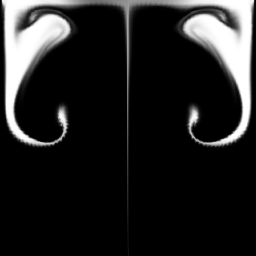
\includegraphics[width=0.23\textwidth]{chap5/L1SR/mean_res256d88}
   \newline  (a) \ \ \ \ \ \ \ \ \ \ \ \ \ \ \ \ \ \ \ \ \ \ \ \ \ \ \ \ \ \ (b) \ \ \ \ \ \ \ \ \ \ \ \ \ \ \ \ \ \ \ \ \ \ \ \ \ \ \ (c) \ \ \ \ \ \ \ \ \ \ \ \ \ \ \ \ \ \ \ \ \ \ \ \ \ \ \ \ \ \ \ (d)
  \bicaption[fig:mean]{重构上采样低频速度场数据}{重构上采样低频速度场数据。(a)、(b)、(c)和(d)分别表示第40、55、62和88帧}{Fig}{fluid simulation result by reconstruction and up-sampling framework, and only the mean part of the velocity filed has been used. (a),(b),(c) and (d) represent for the frame of 40,55,62 and 88.}
\end{figure}

根据L1SR重构上采样方法的具体实现可知,该方法通过双三次插值方法重构上采样流体速度场的低频部分,只有速度场的高频部分通过训练字典方法重构上采样生成。针对实验对比图~\ref{fig:l1sr}表现出的高频部分权重取值越小,其流体形态的左右部分对称性越好的现象,我们推断出如下结论:L1SR方法重构上采样生成的高精度流体速度场高频部分数据的值不够正确,故L1SR重构上采样方法不适宜应用到流体动画领域。

为了让上述推断结论更加具有说服力,我们又做了另外一组实验,即在我们的重构上采样框架中,使用双三次插值方法重构上采样流体速度场的低频部分,去掉L1SR重构上采样的速度场高频部分。图~\ref{fig:mean}展示了该实验的效果图。根据图中展示的效果,可以看出流体速度场数据的低频部分即可形成具有左右对称特点的基本动画形态,但是流体细节丢失严重。结合比较实验~\ref{fig:mean}和~\ref{fig:l1sr},当调整高频部分的系数为 0.5 时,实验生成的流体动画形态存在的不对称问题较为轻微,但是相较于设置高频部分的系数为0.7时的动画效果,其产生的流体细节也相应地减少了很多。再一次证明应用L1SR重构上采样方法到流体动画计算框架中导致的流体动画形态混乱问题,是由其重构速度场与高精度流体速度场之间的误差太大造成的。

分析L1SR方法不能准确重构出原高精度流体速度场的原因,我们发现是由L1SR方法自身存在的理论上不能保证恢复结果的准确性造成的。特别是将该重构方法应用到流体动画计算框架中时,误差会逐帧积累,如果完全不抑制高频部分(实验中取高频部分的系数为0),只需要很少一些帧数之后就会导致流体的形态产生严重的混乱。

\subsubsection{应用scSR重构上采样}

为了提高重构结果的准确性,我们比较了在同一参数条件下,scSR 方法和L1SR方法重构同一幅图像时的峰值信噪比PSNR(Peak Signal to Noise Ratio),如表~\ref{tab:psnr}所示。在此处的实验中,我们也比较了overlap取不同值时的重构结果,无论是从理论的角度,还是根据表中的实验数据,我们都可得这样的结论:重构时使用的overlap值越大,重构效果更好。但是当overlap的值取得越大时,其重构上采样步骤花费的时间也越长。故在我们得流体动画实验中,其overlap值都设置成1。再对比相同参数条件下的scSR方法和L1SR方法的PSNR值,可以发现scSR方法的PSNR值远高于L1SR方法。并且双三次插值重构出的结果的PSNR值也比L1SR方法高。

\begin{table}
  \centering
  \bicaption[tab:psnr]{对比L1SR和scSR方法重构Lena结果图的PSNR值}{对比L1SR和scSR方法重构Lena结果图的PSNR值}{Table}{Comparison of PSNR values of reconstruction result between L1SR and scSR method. }
 \begin{tabular}{|c|c|c|c|} %  cols (left, ctr, right); vert. lines
 \hline % draw horizontal line
 \textbf{reconstruction method} & \textbf{overlap} & $\boldsymbol \lambda$ & \textbf{PSNR values(db)} \\
 \hline
bicubic  &  none & none & 32.794678 \\
 \hline
L1SR   & 1 & 0.15 &  29.689994 \\
scSR &1 &  0.15 & 34.423253 \\
 \hline
L1SR & 4 & 0.15 &  26.55217 \\
scSR &4 &  0.15 &  34.999165\\
 \hline
L1SR   & 1 & 0.2 &  29.470000 \\
scSR &1 &  0.2 & 34.397705 \\
 \hline
L1SR & 4 & 0.2 &  35.011397 \\
scSR &4 &  0.2 &  35.011397\\
\hline
\end{tabular}
\end{table}

\begin{figure}[!ht]
  \centering
  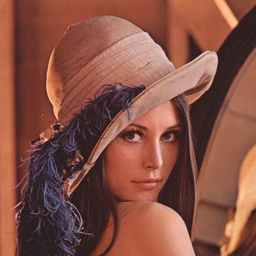
\includegraphics[width=0.45\textwidth]{chap5/scSR/High_pic}
  \hspace{0.1cm}
  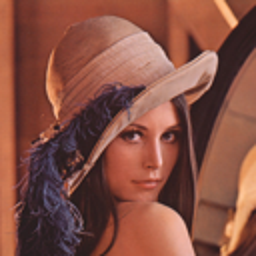
\includegraphics[width=0.45\textwidth]{chap5/scSR/Bic}
  \newline \ \ \ \ \ \ \ \ \ \ \ \ \ (a) high-resolution\ \ \ \ \ \ \ \ \ \ \ \ \ \ \ \ \ \ \ \ \ \ \ \ \ \ \ \ \ \ (b) bicubic\ \ \ \ \ \ \ \ \ \ \ \
  
  \vspace{0.2cm}
  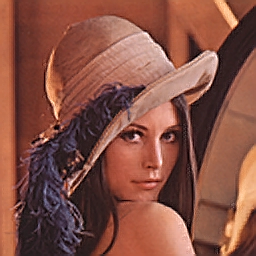
\includegraphics[width=0.45\textwidth]{chap5/scSR/L1SR_p3_o1}
   \hspace{0.1cm}
  \includegraphics[width=0.45\textwidth]{chap5/scSR/scSR_1}
     \newline \ \ \ \ \  \ \ \ \ \ \ \ \ (c) L1SR\ \ \ \ \ \ \ \ \ \ \ \ \ \ \ \ \ \ \ \ \ \ \ \ \ \ \ \ \ \ \ \ \ \ \ \ \ (d) scSR\ \ \ \ \ \ \ \ \ \ \ \ \ 
  \bicaption[fig:l1srVsscSR]{scSR vs L1SR方法重构图像效果图比较}{scSR 与 L1SR方法重构Lena的效果图比较。(a)高精度原图像。(b)双三次插值上采样重构效果。(c)L1SR方法重构效果。(d)scSR方法重构效果}{Fig}{comparison between scSR and L1SR method to reconstruct lena. (a) high-resolution picture. (b) reconstructed by bicubic method. (c) reconstructed by L1SR. (d) reconstructed by scSR.}
\end{figure}

\begin{figure}
  \centering
  
\includegraphics[width=0.13\textwidth]{chap5/scSR/low_res128d20}
  \hspace{0.2cm}
  
\includegraphics[width=0.26\textwidth]{chap5/scSR/bic_res256d20}
   \hspace{0.1cm}
  
\includegraphics[width=0.26\textwidth]{chap5/scSR/scSR_res256d20}
   \hspace{0.1cm}
  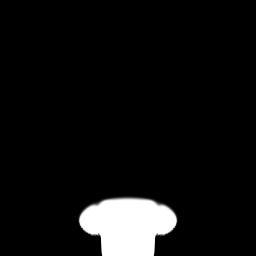
\includegraphics[width=0.26\textwidth]{chap5/scSR/high_res256d20}
  
  \vspace{0.1cm}  
  
\includegraphics[width=0.13\textwidth]{chap5/scSR/low_res128d56}
  \hspace{0.2cm}
  
\includegraphics[width=0.26\textwidth]{chap5/scSR/bic_res256d56}
   \hspace{0.1cm}
  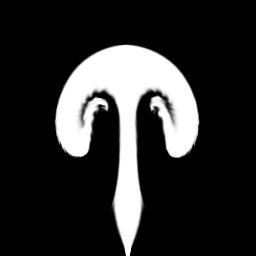
\includegraphics[width=0.26\textwidth]{chap5/scSR/scSR_res256d56}
   \hspace{0.1cm}
  
\includegraphics[width=0.26\textwidth]{chap5/scSR/high_res256d56}
  
    \vspace{0.1cm}  
  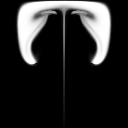
\includegraphics[width=0.13\textwidth]{chap5/scSR/low_res128d73}
  \hspace{0.2cm}
  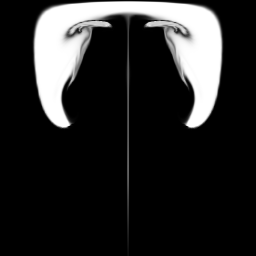
\includegraphics[width=0.26\textwidth]{chap5/scSR/bic_res256d73}
   \hspace{0.1cm}
  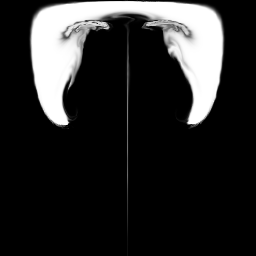
\includegraphics[width=0.26\textwidth]{chap5/scSR/scSR_res256d73}
   \hspace{0.1cm}
  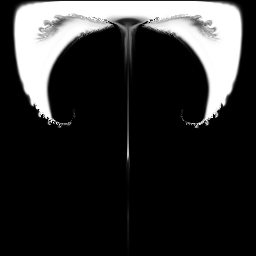
\includegraphics[width=0.26\textwidth]{chap5/scSR/high_res256d73}
  
    \vspace{0.1cm}  
 %  \hspace{0.02cm}
  
\includegraphics[width=0.13\textwidth]{chap5/scSR/low_res128d92}
  \hspace{0.2cm}
  
\includegraphics[width=0.26\textwidth]{chap5/scSR/bic_res256d92}
   \hspace{0.1cm}
  
\includegraphics[width=0.26\textwidth]{chap5/scSR/scSR_res256d92}
   \hspace{0.1cm}
  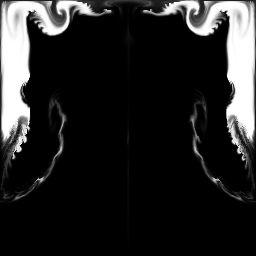
\includegraphics[width=0.26\textwidth]{chap5/scSR/high_res256d92}
   \newline \ (a) \ \ \ \ \ \ \ \ \ \ \ \ \ \ \ \ \ \ \ \ \ \ \ \ \ \ \ \ \ (b) \ \ \ \ \ \ \ \ \ \ \ \ \ \ \ \ \ \ \ \ \ \ \ \ \ \ \ \ \ \ (c) \ \ \ \ \ \ \ \ \ \ \ \ \ \ \ \ \ \ \ \ \ \ \ \ \ \ \ \ (d) \ \ \ \ \ \
  \bicaption[fig:noobs]{无障碍物场景下scSR重构上采样实验结果对比图}{应用scSR重构上采样无障碍物场景下的流体动画模拟框架效果对比图。从上到下的四行分别为第20、56、73和92帧。(a)模拟器直接生成的低精度动画效果。(b)双三次插值上采样重构动画效果。(c)scSR方法重构动画效果。(d)模拟器直接生成的高精度动画效果。}{Fig}{Comparison of applying scSR up-sampling and reconstruction method to fluid animation without obstacles to other simulators. from up to down, the four rows are frames of 20,56,73 and 92.  (a) simulation result on low-resolution MAC grid. (b) simulation result by applying bicubic interpolation to our framework. (c) simulation result by applying scSR method to our framework. (d) simulation result on high-resolution MAC grid.}
\end{figure}

另外,图~\ref{fig:l1srVsscSR}比较了当重叠像素值为1时,L1SR和scSR 方法重构Lena的对比效果图。需要注意的是,图中(c)在重构时取的patch大小为$3\times3$,而(d)则取patch的大小为$5\times5$。这是因为L1SR方法重构图像时,相较于patch大小为$5\times5$,比取patch大小为$3\times3$时的效果更好,其此时其PSNR值为30.355056db。比较图中不同方法的重构效果图,也可以看出scSR方法重构出的结果比L1SR方法更加平滑,但是比双三次插值的结果有更多的细节;而L1SR方法虽然能够重构出一些细节,但是人工痕迹太明显,并且其PSNR值也不及双三次线性插值重构结果的PSNR值。

分析scSR方法与L1SR方法的不同,我们发现,首先,scSR方法对求解稀疏系数的Lasso算法做了一些改进;其次,L1SR方法在做卷积提取高频信息时,辅助使用了一个对低精度输入图像放大2倍后的矩阵,而scSR方法则是直接在放大与放大因子相同倍数的矩阵上做的卷积,这样提取的高频信息更加准确;最后还发现L1SR方法实现论文~\cite{yang2008image}提出的算法时,没有实现重构约束条件的投影步骤,而scSR方法有一个对应的backprojection实现重构约束条件。

在图像超分辨算法中,重构约束条件的目的是为了保证对重构恢复的结果图做下采样和模糊操作,能够得到输入的低精度结果。但是这样的约束条件却并不适用于流体速度场数据,因为流体的低-高精度数据之间没有模糊的关系。故在实验发现scSR方法去掉backprojection步骤后的重构图像的PSNR值仍然要比双三次插值和对应的L1SR方法的PSNR值高时,将修改后的适用于流体速度场数据的scSR方法应用到了我们的流体动画重构上采样框架中。

图~\ref{fig:noobs}展示了在无障碍物的场景下,应用scSR重构上采样方法到我们的流体动画基本框架中的对比效果图。其中,第(a)列是低精度输入速度场数据,第(b)列是应用双三次插值方法到本文提出的流体动画基本框架中的效果图,第(c)列是应用scSR过完备字典技术重构上采样高精度速度场的效果图,第(d)列是模拟器直接在高精度速度场模拟出的效果图。比较(a)、(b)和第(c)列,可以看出这三列的流体形态基本一样,但是在流体的边缘处,应用scSR过完备字典技术重构上采样的流体动画具有一些类似于直接模拟的高精度速度场的细节,其中第92帧最为明显。另外,虽然在流体动画的第20帧,流体形态的出现了明显的不对称,但是当模拟进行到后期,其不对称性问题反而趋于平和。

\begin{figure}
  \centering
  
\includegraphics[width=0.13\textwidth]{chap5/scSR/low_res128d35}
  \hspace{0.2cm}
  
\includegraphics[width=0.26\textwidth]{chap5/scSR/bic_res256d35}
   \hspace{0.1cm}
  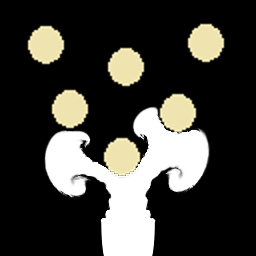
\includegraphics[width=0.26\textwidth]{chap5/scSR/scSR_res256d35}
   \hspace{0.1cm}
  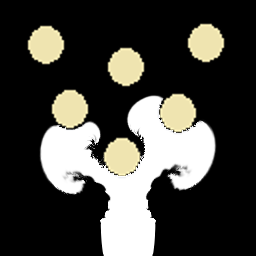
\includegraphics[width=0.26\textwidth]{chap5/scSR/high_res256d35}
  
  \vspace{0.1cm}  
  
\includegraphics[width=0.13\textwidth]{chap5/scSR/low_res128d44}
  \hspace{0.2cm}
  
\includegraphics[width=0.26\textwidth]{chap5/scSR/bic_res256d44}
   \hspace{0.1cm}
  
\includegraphics[width=0.26\textwidth]{chap5/scSR/scSR_res256d44}
   \hspace{0.1cm}
  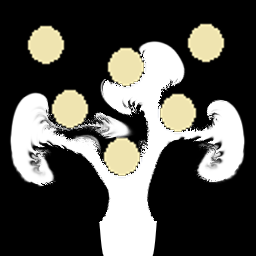
\includegraphics[width=0.26\textwidth]{chap5/scSR/high_res256d44}
  
    \vspace{0.1cm}  
  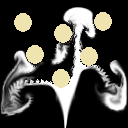
\includegraphics[width=0.13\textwidth]{chap5/scSR/low_res128d55}
  \hspace{0.2cm}
  
\includegraphics[width=0.26\textwidth]{chap5/scSR/bic_res256d55}
   \hspace{0.1cm}
  \includegraphics[width=0.26\textwidth]{chap5/scSR/scSR_res256d55}
   \hspace{0.1cm}
  \includegraphics[width=0.26\textwidth]{chap5/scSR/high_res256d55}
  
    \vspace{0.1cm}  
 %  \hspace{0.02cm}
  \includegraphics[width=0.13\textwidth]{chap5/scSR/low_res128d70}
  \hspace{0.2cm}
  \includegraphics[width=0.26\textwidth]{chap5/scSR/bic_res256d70}
   \hspace{0.1cm}
  \includegraphics[width=0.26\textwidth]{chap5/scSR/scSR_res256d70}
   \hspace{0.1cm}
  \includegraphics[width=0.26\textwidth]{chap5/scSR/high_res256d70}
   \newline \ (a) \ \ \ \ \ \ \ \ \ \ \ \ \ \ \ \ \ \ \ \ \ \ \ \ \ \ \ \ \ (b) \ \ \ \ \ \ \ \ \ \ \ \ \ \ \ \ \ \ \ \ \ \ \ \ \ \ \ \ \ \ (c) \ \ \ \ \ \ \ \ \ \ \ \ \ \ \ \ \ \ \ \ \ \ \ \ \ \ \ \ (d) \ \ \ \ \ \
  \bicaption[fig:obs]{多障碍物场景下scSR重构上采样实验结果对比图}{应用scSR重构上采样多障碍物场景下的流体动画模拟框架效果对比图。从上到下的四行分别为第35、44、55和70帧。(a)模拟器直接生成的低精度动画效果。(b)双三次插值上采样重构动画效果。(c)scSR方法重构动画效果。(d)模拟器直接生成的高精度动画效果。}{Fig}{Comparison of applying scSR up-sampling and reconstruction method to fluid animation with multi-obstacles to other simulators. from up to down, the four rows are frames of 35,44,55 and 70.  (a) simulation result on low-resolution MAC grid. (b) simulation result by applying bicubic interpolation to our framework. (c) simulation result by applying scSR method to our framework. (d) simulation result on high-resolution MAC grid.}
\end{figure}

\begin{figure}
  \centering
  \includegraphics[width=0.13\textwidth]{chap5/low_dens_68}
  \hspace{0.2cm}
  \includegraphics[width=0.26\textwidth]{chap5/bic_dens_68}
   \hspace{0.1cm}
  \includegraphics[width=0.26\textwidth]{chap5/scSR_dens_68}
   \hspace{0.1cm}
  \includegraphics[width=0.26\textwidth]{chap5/high_dens_68}
  
  \vspace{0.1cm}  
  \includegraphics[width=0.13\textwidth]{chap5/low_dens_106}
  \hspace{0.2cm}
  \includegraphics[width=0.26\textwidth]{chap5/bic_dens_106}
   \hspace{0.1cm}
  \includegraphics[width=0.26\textwidth]{chap5/scSR_dens_106}
   \hspace{0.1cm}
  \includegraphics[width=0.26\textwidth]{chap5/high_dens_106}
  
    \vspace{0.1cm}  
  \includegraphics[width=0.13\textwidth]{chap5/low_dens_179}
  \hspace{0.2cm}
  \includegraphics[width=0.26\textwidth]{chap5/bic_dens_179}
   \hspace{0.1cm}
  \includegraphics[width=0.26\textwidth]{chap5/scSR_dens_179}
   \hspace{0.1cm}
  \includegraphics[width=0.26\textwidth]{chap5/high_dens_179}
  
    \vspace{0.1cm}  
 %  \hspace{0.02cm}
  \includegraphics[width=0.13\textwidth]{chap5/low_dens_249}
  \hspace{0.2cm}
  \includegraphics[width=0.26\textwidth]{chap5/bic_dens_249}
   \hspace{0.1cm}
  \includegraphics[width=0.26\textwidth]{chap5/scSR_dens_249}
   \hspace{0.1cm}
  \includegraphics[width=0.26\textwidth]{chap5/high_dens_249}
   \newline \ (a) \ \ \ \ \ \ \ \ \ \ \ \ \ \ \ \ \ \ \ \ \ \ \ \ \ \ \ \ \ (b) \ \ \ \ \ \ \ \ \ \ \ \ \ \ \ \ \ \ \ \ \ \ \ \ \ \ \ \ \ \ (c) \ \ \ \ \ \ \ \ \ \ \ \ \ \ \ \ \ \ \ \ \ \ \ \ \ \ \ \ (d) \ \ \ \ \ \
  \bicaption[fig:obsscSR]{C++模拟器中应用scSR重构上采样实验结果对比图}{C++模拟器中应用scSR重构上采样实验结果对比图。从上到下的四行分别为第68、106、179和249帧。(a)模拟器直接生成的低精度动画效果。(b)双三次插值上采样重构动画效果。(c)scSR方法重构动画效果。(d)模拟器直接生成的高精度动画效果。}{Fig}{Comparison of applying scSR up-sampling and reconstruction method to fluid animation developed with c++. from up to down, the four rows are frames of 68,106,179 and 249.  (a) simulation result on low-resolution MAC grid. (b) simulation result by applying bicubic interpolation to our framework. (c) simulation result by applying scSR method to our framework. (d) simulation result on high-resolution MAC grid.}
\end{figure}

类似于图~\ref{fig:noobs},图~\ref{fig:obs}展示的是在多障碍物的场景下,基于过完备训练字典的scSR重构方法的对比效果图。比较图中的第(a)、(b)和第(c)列,我们可以得出与图~\ref{fig:noobs}一样的结论。在通过上述实验验证后,我们可以总结出结论:应用过完备稀疏字典技术的重构上采样方法,能够在一定程度上重构出类似与高精度网格模拟器生成的流体细节效果,但是模拟出的流体动画的形态更接近于低精度的模拟结果,并且重构生成的流体动画还存在一些形态性问题。

\section{应用降采样矩阵的重构上采样方法}

\subsection{实验背景}

本文提出流体动画重构上采样框架,目的是为了达到快速高效地模拟流体动画的目的。但是,应用scSR方法在Matlab环境下重构上采样流体速度场,即使overlap值设置为1,其重构上采样步骤的时间开销也需要约$1.5~1.7s$每帧,如果增加局部细微结构之间的overlap值,其重构上采样步骤耗费的时间会更长。但是在同样的条件下,双三次插值方法却只需要花费大约$0.003s$每帧。

为了提高上述实验中scSR重构方法的在流体速度场重构上采样步骤中的时间开销,并且验证该方法的通用性,我们更换了一个C++模拟器,并将scSR方法应用到了C++开发环境中。在实验的过程中,模拟器中上升的烟雾柱较小,计算产生的误差效果将会更加突出。应用scSR方法到C++模拟器中后,我们发现不对称性问题及形态问题十分突出,如图~\ref{fig:obsscSR}所示。

\subsection{实验目的与环境}

 分析应用过完备训练字典的scSR方法在流体动画上存在的问题,我们发现从本质上来讲,无论是scSR方法还是L1SR方法,都存在求解稀疏系数时,训练字典的最优空间和重构上采样的最优空间不一致问题,从理论上讲,不能保证重构结果的准确性。虽然这些算法能够在图像超分辨领域取得令人满意的结果,但是不能保证其在流体动画中也能取得好的效果。图像超分辨领域,只要单张的重构结果在视觉上能让人满意即可,但是在流体模拟领域,如果重构结果存在误差,该误差会逐帧积累,最终导致流体的形态产生严重的问题。应用降采样矩阵的重构上采样方法是为了从本质上克服基于稀疏编码的过完备字典方法的空间不一致问题而提出的。
 
 在应用降采样矩阵的重构上采样方法的实验中,我们使用的电脑内核为Intel Core i7 3.40GHz,内存为16G。在应用本文提出的降采样矩阵的重构方法到流体动画领域之前,我们在图像处理领域验证其重构结果的准确度。在学习高精度的训练字典时,我们设流体速度场数据的训练样本的局部细微结构patch大小为$8\times8$,放大因子仍然为2,则重构时使用的低精度速度场的patch大小的为$4\times4$。根据上述实验参数的设定,我们可推断出高精度空间字典的原子项向量有64个值,对应低精度空间字典的原子项向量为16个值,那么降采样矩阵$\boldsymbol S$的维度为$16 \times 64$,实验中我们使用的是双线性插值采样矩阵。拉格朗日算子$\lambda$的值设为1。根据基于稀疏编码的过完备字典技术,我们知道字典越大,其重构效果越好。但是其重构步骤的开销也会线性增长。为了平衡重构效果与重构的时间开销,在我们的实验中,我们仍然使用的字典大小为256。
 
 在实验中,我们使用的是在C++环境下开发的模拟器,不同于在Matlab环境中实验用的模拟器,在应用降采样矩阵的重构上采样方法的实验中,我们在流体模拟的基本步骤-对流步骤中使用的Maccormack~\cite{selle2008unconditionally}方法,投影步骤的矩阵线性方程使用的pcg求解器。
 
\subsection{实验结果与分析}

\begin{figure*}[]
 \center
 \includegraphics[height=1.85 in]{chap5/lena_res.png}
 \bicaption[fig:lena]{应用降采样矩阵的重构上采样方法重构Lena}{应用降采样矩阵的重构上采样方法重构Lena}{Fig}{Super-resolution result for lena by using down-sampling matrix. Left:bicubic. center:our method. right:orginal picture.}
\end{figure*}

\begin{figure*}[]
 \center
% \includegraphics[height=1.6 in]{images/40compare.png}
 \includegraphics[height=1.43 in]{chap5/obs_16_40.png}
 \newline \includegraphics[height=1.43 in]{chap5/obs_8_60.png}
 \newline \includegraphics[height=1.43 in]{chap5/obs_16_200.png}
  \newline \includegraphics[height=1.43 in]{chap5/obs_16_240.png}
\newline  (a) \ \ \ \ \ \ \ \ \ \ \ \ \ \ \ \ \ \ \ \ \ \ \ \ \ \ \ \ \ \ (b) \ \ \ \ \ \ \ \ \ \ \ \ \ \ \ \ \ \ \ \ \ \ \ \ \ \ \ (c) \ \ \ \ \ \ \ \ \ \ \ \ \ \ \ \ \ \ \ \ \ \ \ \ \ \ \ \ \ \ \ (d)
 \bicaption[fig:no_obs]{应用降采样矩阵的重构上采样方法重构流体动画}{(a)模拟器模拟的低精度结果\(128 \times 128\)。(b)通过上三次插值方法重构上采样到 \(256 \times 256\) 。(c)通过降采样矩阵的字典方法重构上采样到 \(256 \times 256\) 。(d)模拟器模拟的高精度结果 \(256 \times 256\) }{Fig}{(a) \(128 \times 128\) simulation result of low-resolution. (b) up-sampling to \(256 \times 256\) by bicubic. (c) up-sample to \(256 \times 256\) by down-sampling and dictionaries method. (d) \(256 \times 256\) simulation result of high-resolution.}
\end{figure*}

图~\ref{fig:lena}展示了本文提出的重构方法重构lena图片的效果图。观察图中的效果可知,本文方法可以重构出比双三次插值更多的细节效果,并且在本文方法重构出的结果图中,几乎没有人工痕迹。为了让我们的实验更具有说服力,我们同样记录了重构结果的PSNR值。其中,双三次插值重构结果的PSNR值为33.018db,而我们方法重构结果的PSNR值能达到34.285db。

如图~\ref{fig:no_obs}所示,从(a)到(d)依次为低精度网格模拟的动画效果、上三次插值上采样、降采样矩阵的字典方法重构上采样和高精度网格模拟的动画效果。观察图中动画效果,可以看出双三次插值重构上采样生成的动画丢失了很多细节,而降采样矩阵的训练字典方法则能恢复一些与高精度网格模拟出的动画类似的涡旋细节,但是其流体的形态却介于低-高精度的模拟结果之间。

\begin{figure*}
 \center
 \includegraphics[height=1.43 in]{chap5/obs40.png}
%\newline \includegraphics[height=1.43 in]{chap5/obs60.png}
 \includegraphics[height=1.43 in]{chap5/obs160.png}
 \newline \includegraphics[height=1.43 in]{chap5/obs180.png}
\newline  (a) \ \ \ \ \ \ \ \ \ \ \ \ \ \ \ \ \ \ \ \ \ \ \ \ \ \ \ \ \ \ (b) \ \ \ \ \ \ \ \ \ \ \ \ \ \ \ \ \ \ \ \ \ \ \ \ \ \ \ (c) \ \ \ \ \ \ \ \ \ \ \ \ \ \ \ \ \ \ \ \ \ \ \ \ \ \ \ \ \ \ \ (d)
 \bicaption[fig:downobs]{应用降采样矩阵的字典方法重构上采样方法重构有障碍物场景的流体动画}{(a)模拟器模拟的低精度结果\(128 \times 128\)。(b)通过上三次插值方法重构上采样到 \(256 \times 256\) 。(c)通过降采样矩阵且patch大小为\((8 \times 8)\)的字典方法重构上采样到 \(256 \times 256\) 。(d)模拟器模拟的高精度结果 \(256 \times 256\) }{Fig}{(a):\(128 \times 128\) simulation result. (b): up-sampling to \(256 \times 256\) by bicubic. (c): up-sampling to \(256 \times 256\) by dictionaries method \((8 \times 8)\). (d): \(256 \times 256\) simulation result.}
\end{figure*}

图~\ref{fig:downobs}给我们展示的是在有障碍物的情况下应用降采样矩阵的字典方法重构生成的流体动画。对比各动画效果图,我们可以得出与无障碍物的场景一样的结论,即应用降采样的过完备训练字典方法能够在一定程度上重构出高精度流体的细节。仔细观察我们可以发现相较于高精度网格的流体动画,通过双三次插值上采样生成的流体动画效果的能量损耗很严重,因为其在相同帧的情况下,高精度网格生成的动画的烟雾上升的高度远高于上三次上采样重构出的动画的烟雾的高度,并且烟雾的耗散也较为严重。但是本文提出的重构方法则好很多。相反,本文方法重构出的动画的烟雾甚至比高精度模拟出来的更多一些。

\begin{table}
  \centering
  \bicaption[tab:time_table]{降采样训练字典方法的重构时间}{降采样训练字典方法的重构时间}{Table}{computation times of down-samping dictionaries .}
 \begin{tabular}{|c|c|c|} %  cols (left, ctr, right); vert. lines
 \hline % draw horizontal line
 \textbf{method} & \textbf{grid} & \textbf{computation time(s/frame)} \\
 \hline
low-resolution  &  \(128 \times 128\) & 0.046 \\
 \hline
bicubic   & \(256 \times 256\)  &  0.127 \\
 \hline
dictionaries\((8 \times 8)\) & \(256 \times 256\) &  1.68 \\
 \hline
 dictionaries\((16 \times 16)\) &  \(256 \times 256\) &  0.24 \\
 \hline
 high-resolution  &  \(256 \times 256\) &  0.276 \\
\hline
\end{tabular}
\end{table}

表格~\ref{tab:time_table}列出了在图~\ref{fig:downobs}中所示的各种流体模拟方法,以及降采样过完备稀疏字典方法在使用不同的patch大小时,每帧的计算开销。比较表格中低精度网格和高精度网格的时间开销,我们可知,即使网格的放大因子只为2,但是时间开销却增加了6倍。另外,我们实现的C++版本模拟器本身就是一个运行效率比较高的模拟器,可从表中数据看出,当我们使用大小为\((8 \times 8)\)的流体局部细微结构时,应用本文提出的重构上采样计算框架没有加速的空间。但是如果将我们的重构上采样流体动画计算框架应用到其他较慢的模拟器中,可以达到加速的目的,因为无论使用什么样的模拟器,我们的重构方法的时间开销是固定的。如果我们把表示流体局部细微结构的patch的大小改成\((16 \times 16)\),即使是与该计算效率较高的模拟器相比,我们的重构上采样方法的计算速度也能比高精度网格的模拟器稍快一些。

\begin{figure*}
 \center
 \includegraphics[height=1.43 in]{chap5/obs_16_60.png}
\newline \includegraphics[height=1.43 in]{chap5/obs_16_120.png}
\newline  (a) \ \ \ \ \ \ \ \ \ \ \ \ \ \ \ \ \ \ \ \ \ \ \ \ \ \ \ \ \ \ (b) \ \ \ \ \ \ \ \ \ \ \ \ \ \ \ \ \ \ \ \ \ \ \ \ \ \ \ (c) \ \ \ \ \ \ \ \ \ \ \ \ \ \ \ \ \ \ \ \ \ \ \ \ \ \ \ \ \ \ \ (d)
 \bicaption[fig:obs_16]{对流体速度场选择性地应用过完备训练字典技术}{(a)使用双三次上采样方法重构的流体动画。(b)使用patch大小为\((16 \times 16\)的过完备训练字典技术重构的流体动画。(c)选择性地使用patch大小为\((16 \times 16\)的过完备训练字典技术重构的流体动画。(d)直接模拟的\(256 \times 256\)高精度动画效果。}{Fig}{(a):up-sampling to \(256 \times 256\) by bicubic result. (b): up-sample to \(256 \times 256\) by dictionaries method \((16 \times 16)\). (c): up-sample to \(256 \times 256\) by dictionaries method \((16 \times 16)\) with a bicubic interpolation to accelerate. (d): \(256 \times 256\) simulation result.}
\end{figure*}

另外,我们可以选择性地将过完备训练字典技术应用到速度场中,即只应用基于稀疏编码技术的过完备字典技术到有大量烟雾填充的局部细微结构中,而使用更加快速的上采样方法重构上采样其他局部细微结构,比如双三次插值上采样方法,这样可以在很大程度上提高流体模拟的速度,但是又不损失流体模拟的质量。如图~\ref{fig:obs_16}所示,比较了在完全应用以及选择性应用局部细微结构patch大小为\((16 \times 16)\)到本文提出的重构上采样计算框架上的效果。比较第(a)列和第(b)列,可以看出应用基于稀疏编码的过完备字典技术的效果远好于使用双三次上采样重构上采样的效果,再比较第(b)列和第(c)列,可以看出选择性地应用过完备训练字典技术与完全使用过完备训练字典技术到流体模拟框架中的动画效果几乎一样,而在最初几帧,选择性地应用过完备训练字典技术的时间开销只有0.13s每帧左右。

\section{本章小结}

首先,我们应用L1SR重构方法到本文提出的重构上采样基本框架中,验证本课题的可行性。但是从实验的结果看出,本文提出的重构上采样方法与框架能在一定程度上重构出类似于高精度网格速度场的涡旋细节,但是其模拟出的流体动画形态问题较大;其后我们又应用scSR重构上采样方法到本文提出的模拟框架中,该重构方法的动画效果虽然有所改善,但是因为scSR重构上采样方法并没有从根本上解决L1SR方法存在的问题,故在使用C++模拟器之后,流体的形态问题又暴露了出来;最后,针对L1SR方法和scSR方法存在的共同问题,本文提出了应用降采样矩阵的过完备训练字典技术,并对比了该重构算法与双三次插值重构上采样方法的重构效果,可以看出本文提出的应用降采样矩阵的稀疏训练字典方法的计算框架能够重构出更多的流体细节,并且也不存在应用双三次重构上采样方法时存在的能量耗散问题。

其次,如果以计算速度较慢的模拟器作为本文提出的重构上采样方法的基本模拟方法,本文方法能够在一定程度上提高模拟的速度;即使是以本文中使用的计算效率较高的C++模拟器作为基本模拟方法,也可以通过增加流体局部细微结构的大小,或者选择性地应用基于稀疏编码的过完备训练字典方法,达到提高流体计算速度的目的。

